% !TeX root = ../main.tex

\chapter{CE$\nu$NS探测研究背景}

\section{CE$\nu$NS过程}

\begin{figure}
    \centering
    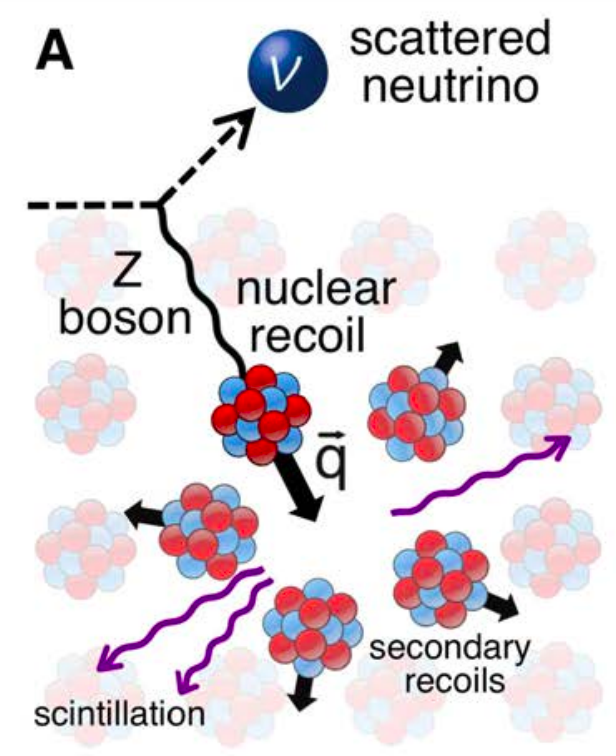
\includegraphics[width=0.4\linewidth]{figures/CEvNS_demo.png}
    \caption{\label{fig:cevns_demo} 中微子-原子核相干弹性散射示意图}
\end{figure}

CE$\nu$NS是中微子和原子核之间的弹性中性流相互作用,于1974年被首次预言提出\cite{freedman_coherent_1974,kopeliovich_isotopic_1974}。
如图\ref{fig:cevns_demo},中微子与原子核交换Z玻色子,同时也交换能量动量,产生核反冲(nuclear recoil, NR)。
被加速的原子核以闪烁光(scintillation)和二次碰撞(secondary recoils)的形式继续将能量沉积到周围的物质中,
最终这些信号被探测器记录到\cite{akimov_observation_2017}。在中微子和原子核交换Z玻色子的过程中,若动量转移足够小,
则原子核近似作为一个整体与中微子作用,作用截面近似与原子核中的中子个数的平方成正比关系。

\begin{align}
    \label{eq:cevns}
    \frac{\mathrm{d}\sigma(E_\nu)}{\mathrm{d}T} &= \frac{G_F^2 M}{2\pi}\left[(G_V+G_A)^2+(G_V-G_A)^2(1-\frac{T}{E_{\nu}})^2-(G_V^2-G_A^2)\frac{MT}{E_{\nu}^2}\right] \\
    G_V &= (g_V^p Z+g_V^n N)F^V(Q^2) \\
    G_A &= (g_A^p(Z_{+}-Z_{-})+g_A^n(N_{+}-N_{-}))F^A(Q^2) \\
    \label{eq:cevns_theta}
    g_V^p &= \rho_{\nu N}^{NC}(\frac{1}{2} - 2\hat{\kappa}_{\nu N}\sin^2\theta_W) + 2\lambda^{uL} + 2\lambda^{uR} + \lambda^{dL} + \lambda^{dR} \\
    g_V^n &= -\frac{1}{2}\rho_{\nu N}^{NC} + \lambda^{uL} + \lambda^{uR} + 2\lambda^{dL} + 2\lambda^{dR}
\end{align}

公式\ref*{eq:cevns}为具有特定能量$E_{\nu}$的电子反中微子与特定质量$M$的原子核的CE$\nu$NS微分截面,
其中$T$为末态原子核动能,$G_F$为费米常数(Fermi constant),本文中取为1.1664$\times10^{-5}\si{GeV}^{-2}$,$Q$为动量转移,$Z$和$N$分别为原子核内质子和中子的个数。
$F^V$和$F^A$为形状因子,在低动量转移下可以认为$F^V(Q^2)=F^A(Q^2)=1$\cite{lewin_review_1996},
$\rho_{\nu N}^{NC},\hat{\kappa}_{\nu N}$为弱电理论参数,
$\lambda^{uL},\lambda^{uR},\lambda^{dL},\lambda^{dR}$是辐射校正参数\cite{barranco_probing_2005}。
$Z_{\pm}$和$N_{\pm}$是原子核内自旋(spin)取向为上($+$)和下($-$)的质子和中子个数。

经过计算,$|g_V^p|\ll|g_V^n|$,所以在 $G_V$ 参数中起主要作用的因素是中子个数 $N$;
另一方面,根据原子核物理理论,对于偶偶核(even-even nucleus),即原子核内质子数$Z$和中子数$N$均为偶数时,$Z_{+}=Z_{-},N_{+}=N_{-}$。
届时 $G_A=0$,我们可以利用这一点将CE$\nu$NS截面简化。

\begin{align}
    \label{eq:cevns_even_even}
    \frac{\mathrm{d}\sigma(E_\nu)}{\mathrm{d}T} &= \frac{G_F^2 M}{2\pi}G_V^2\left[1+(1-\frac{T}{E_{\nu}})^2-\frac{MT}{E_{\nu}^2}\right] \\
    G_V &= (g_V^p Z+g_V^n N)F^V(Q^2)
\end{align}

公式\ref{eq:cevns_even_even}为CE$\nu$NS截面的的偶偶核简化形式。考虑到 $|g_V^p|\ll|g_V^n|$,则$G_V^2\approx N^2$,
最后可以近似得到$\frac{\mathrm{d}\sigma(E_\nu)}{\mathrm{d}T}\approx N^2$,对于非偶偶核,该式也近似成立。这正是CE$\nu$NS相干性的体现。

对于不同种类的核素,因为原子核的质量$M$不同,所以微分截面$\frac{\mathrm{d}\sigma(E_\nu)}{\mathrm{d}T}$不同。
将微分截面对原子核末态动能$T$积分,可以得到CE$\nu$NS总截面随着中微子能量$E_{\nu}$的变化关系。

\begin{figure}
    \centering
    \includesvg[width=0.6\linewidth]{figures/cross_section.svg}
    \caption{\label{fig:xsec_elements} CE$\nu$NS对各种核素的截面随着中微子能量$E_{\nu}$的变化关系}
\end{figure}

图\ref{fig:xsec_elements}中列举了几种探测器常用核素(元素)的CE$\nu$NS截面与$E_{\nu}$的关系。作为对比,图中还包括了IBD\cite{akimov_observation_2017}的截面以及中微子-电子相干弹性散射(neutrino-electron elastic scattering, E$\nu$ES)的截面随着$E_{\nu}$的变化。
几种截面都随着中微子能量升高而升高,但几种CE$\nu$NS截面始终高于IBD和与电子相互作用的截面。同时对于更重的元素,如$\mathrm{Xe}$,CE$\nu$NS截面相比于其他较轻元素更大。
从截面大小的角度看,CE$\nu$NS相比IBD更容易被探测;但是因为CE$\nu$NS的动量转移太小,且不同于IBD可以借助$\gamma$和中子进行事件标记,对CE$\nu$NS的成功探测远晚于IBD。
同时图\ref{fig:xsec_elements}也为我们提示了选择探测器材料的思路:重元素的反应截面更大,对探测更有利。但是考虑到原子核末态动能也会随着元素质量数增加而偏向更低能量,
以及不同探测器介质下探测器技术和性能的差异,应综合考虑选择探测手段。

\section{CE$\nu$NS探测方法与进展}

2017年,COHERENT合作组在美国橡树岭实验室的散射中子源上使用$\mathrm{CsI}$以高置信度探测到了$\pi$介子(pion)衰变过程放出的中微子的CE$\nu$NS信号\cite{akimov_observation_2017}。
此后他们又并行开展了以其他手段进行CE$\nu$NS搜寻的实验,其中包括了HPGe、单相液氩(single phase LAr)探测器和碘化钠($\mathrm{NaI}$)。
虽然这些探测器的能量阈值不尽相同,但得益于散裂中子源中微子的较高能量($\mathcal{O}\left(10\si{MeV}\right)$),
CE$\nu$NS在这些探测器中的NR可以达到$\mathcal{O}\left(10\si{keV}\right)$,探测器阈值并不是实验成败的最关键因素。

目前有多个合作组及实验正在进行CE$\nu$NS探测研究,除COHERENT外均使用反应堆中微子作为中微子源。
表\ref{tab:experiments}列出了部分CE$\nu$NS探测研究的相关实验,但目前没有实验成功给出测量到反应堆中微子CE$\nu$NS的结果。

\begin{table}
  \centering
  \caption{从事CE$\nu$NS探测研究的相关实验}
  \begin{tabular}{ccc}
    \toprule
    实验名称 & 探测器材料 & 研究进展 \\
    \midrule
    COHERENT & $\mathrm{CsI,HPGe,LAr,NaI}$ & 进行中\cite{coherent_collaboration_monitoring_2022} \\
    CONUS & $\mathrm{Ge}$ 低温量能器 & 进行中\cite{conus_collaboration_novel_2021} \\
    CONNIE & $\mathrm{CCD}$ & 进行中\cite{connie_collaboration_search_2022} \\
    MINER & $\mathrm{Ge}$ 低温量能器 & 筹划中\cite{agnolet_background_2017} \\
    \bottomrule
  \end{tabular}
  \label{tab:experiments}
\end{table}

反应堆中微子CE$\nu$NS的低动量转移特性要求探测器实现极低阈值和低能区域的极低本底。
类似的要求也在在相关领域,如暗物质直接探测,成为探测器关键技术。低质量暗物质,如$\mathcal{O}\left(1\si{GeV}\right)$大质量弱相互作用粒子(Weakly interacting massive particles, WIMP)对探测器原子核的核反冲动量转移也在几个$\si{keV}$量级。
目前流行的暗物质探测技术中,LXeTPC和HPGe探测器均取得了较先进的成果。用于探测WIMP的探测器技术同样可以应用到同为核反冲信号的CE$\nu$NS探测中。
因反应堆均在地面附近,若设计建造一台能够在地面正常运行的LXeTPC或HPGe探测器,则有可能实现对反应堆中微子CE$\nu$NS的探测。
